\chapter{Testing and Results}
\label{results}
\index{Testing and Results%
	@\emph{Testing and Results}}%

In order to test the effectiveness of Honeycomb as an indoor location estimation tool, we ran a series of tests variants in a single location and mapped out the results for comparison. In this section we present the testing setup and the results. 


\section{Testing Setup}
\index{Testing Setup@\emph{Testing Setup}}%

 A map of our location can be seen in Figure \ref{loc1_path}. This space is roughly 24 feet wide by 42 feet long for a total of approximately 1000 square feet. The dotted line in the figure represents our actual route through the space, which we repeated for each test variant. The shaded areas and dark lines are walls or other inaccessible areas in the actual location, although they could just as easily represent shelving or other displays in the grocery store scenario. The solid black dots are our fingerprint locations.
 
 We employed six Wi-Fi access points of various makes and models for our testing. TODO: makes and models here. We chose these access points because they are popular brands which can be found in wide use today, and thus represent a real world scenario. Our mobile device, both for fingerprinting and user track collection was a Samsung Galaxy S5. 
 
 Unlike much of the location estimation research in this area, we did not make a regularly spaced grid of fingerprints, choosing instead to place fingerprints only at notable locations in the space. This does decrease precision slightly, but also makes the fingerprinting process less painful, which is an important factor in adoption in a real world deployment. However, even with fingerprints only at notable locations, a sufficient density of fingerprints will still provide an adequate level of precision for our intended scenarios. In our tests, we placed 10 fingerprints in a 1000 square foot space, which is roughly one fingerprint for every 10 square feet. In the scenarios that we described in chapter \ref{introduction}, we believe that would be adequate precision. 


\begin{figure}[htb] % Imported eps example.
	\centering
	\ 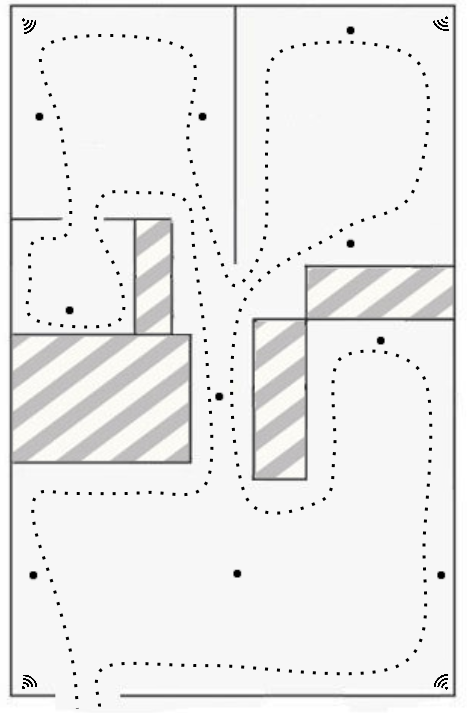
\includegraphics[width=2.8in,height=4in]{loc1_path.png}
	\caption{Map of location, with fingerprint points and walking path}
	\label{loc1_path}
\end{figure}

\section{Test Variants}
\index{Test Variants@\emph{Test Variants}}%


While there are many possible variables that could be tested, from Wi-Fi access point signal reliability to individual mobile phone capabilities, the two main variables that are most relevant to viability of Honeycomb are the number of access points in the space and the length of the poll time for each fingerprint.

The importance of the number of access points in the space is obvious. We make an assumption in our tests that a single access point, or even two or three access points, is simply not enough to get a reliable estimation. Therefore, we introduced two major test variants, one with four access points and one with six. 

The less obvious, but potentially more crucial variable is the length of time spent polling each fingerprint location. As described in chapter \ref{tech-overview}, Honeycomb is capable of taking multiple signal strength measurements for each fingerprint location so as to avoid incorrect measurements due to abnormally large or small instantaneous values. The question, then, is what amount of time spent polling a single fingerprint is enough to get an accurate measurement. Therefore, we introduced three test variants for polling time: 10 seconds, 20 seconds, and 30 seconds.

Thus, with these two variables and their variants, we have six independent tests: four and six access points, each with polling times of 10, 20, and 30 seconds. For the four access point tests, we placed an access point at each of the four corners of the space, and for the six access point tests, we placed two additional access points at the mid point of the longer walls on either side. For each test we independently fingerprinted the entire space, and then talked the route mapped out in Figure \ref{loc1_path}.


\section{Results}
\index{Results@\emph{Results}}%


Figures \ref{loc1_4ap_10s}, \ref{loc1_6ap_10s}, \ref{loc1_4ap_20s}, \ref{loc1_6ap_20s}, \ref{loc1_4ap_30s}, and \ref{loc1_6ap_30s} represent the results of each of our test variants. In these maps, we have placed a large red dot at the fingerprint which represents the first estimation of the user's location. From there, we have placed numbered red lines to each of the subsequent fingerprint locations estimated to be the user's location. It is important to note that these lines are not intended to represent the user's actual movement through the space, but are simply handy references for showing general movement from one fingerprint area to another. As such, these lines are free to move through walls, and can be either straight or curved, depending on need.  It is also important to note that the number of lines in each map can vary significantly, due to the fact that the same fingerprint location can be considered the user's location at multiple successive timestamps, and we have only represented instances of location change in these result maps. 


\begin{figure}
	\centering
	\begin{minipage}{0.45\textwidth}
		\ 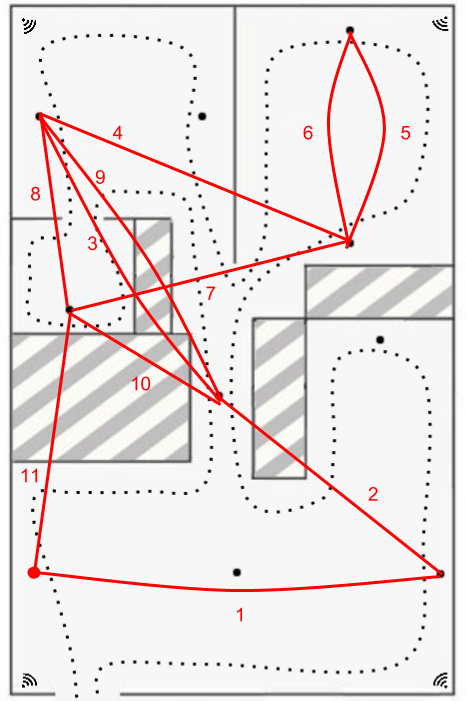
\includegraphics[width=2in,height=2.8in]{loc1_4ap_10s.png}
		\caption{Results with four access points and a ten second polling time}
		\label{loc1_4ap_10s}
	\end{minipage}\hfill
	\begin{minipage}{0.45\textwidth}
		\centering
		\ 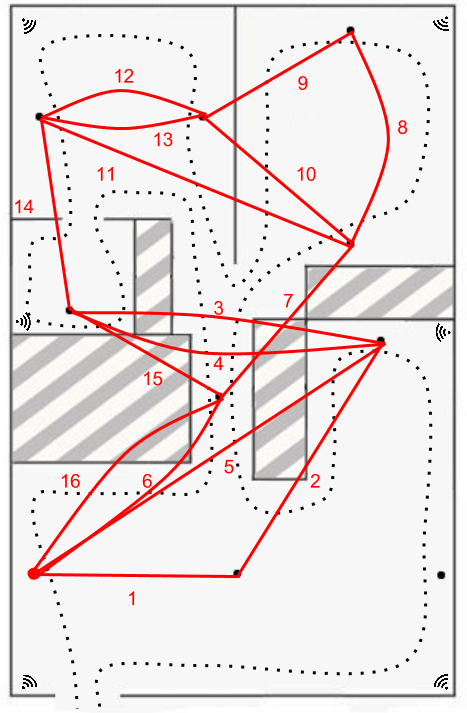
\includegraphics[width=2in,height=2.8in]{loc1_6ap_10s.png}
		\caption{Results with six access points and a ten second polling time}
		\label{loc1_6ap_10s}
	\end{minipage}
\end{figure}

\begin{figure}
	\centering
	\begin{minipage}{0.45\textwidth}
		\ 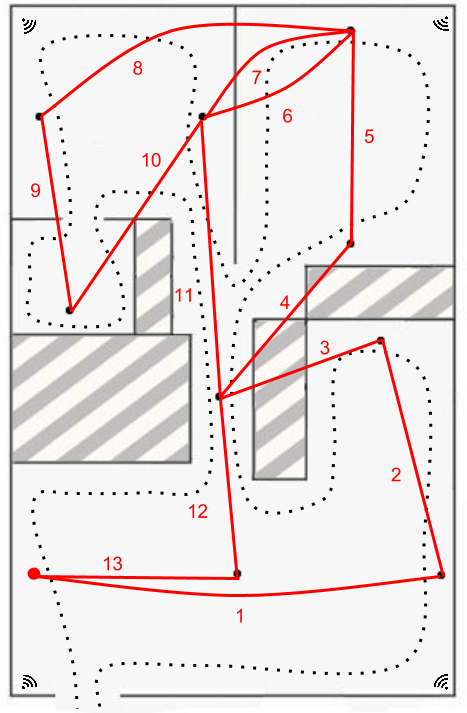
\includegraphics[width=2in,height=2.8in]{loc1_4ap_20s.png}
		\caption{Results with four access points and a twenty second polling time}
		\label{loc1_4ap_20s}
	\end{minipage}\hfill
	\begin{minipage}{0.45\textwidth}
		\centering
		\ 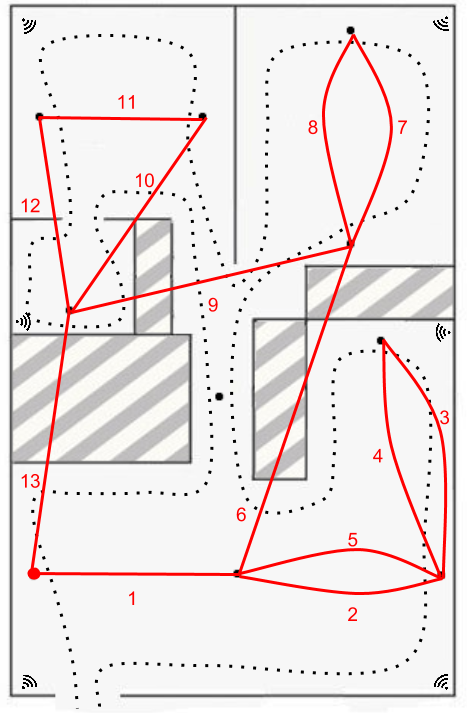
\includegraphics[width=2in,height=2.8in]{loc1_6ap_20s.png}
		\caption{Results with six access points and a twenty second polling time}
		\label{loc1_6ap_20s}
	\end{minipage}
\end{figure}

\begin{figure}
	\centering
	\begin{minipage}{0.45\textwidth}
		\ 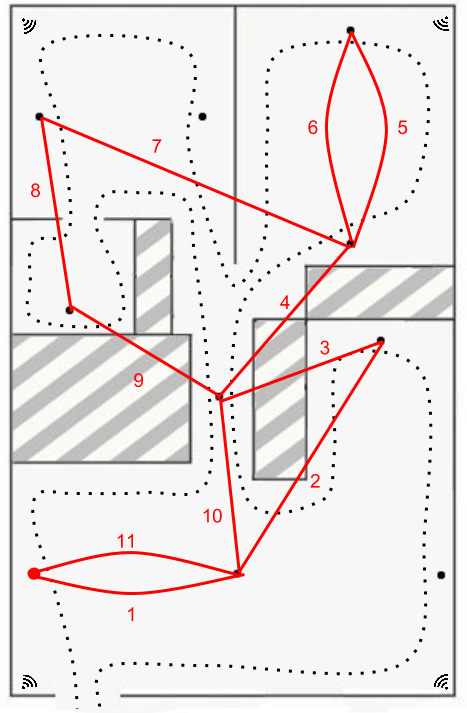
\includegraphics[width=2in,height=2.8in]{loc1_4ap_30s.png}
		\caption{Results with four access points and a thirty second polling time}
		\label{loc1_4ap_30s}
	\end{minipage}\hfill
	\begin{minipage}{0.45\textwidth}
		\centering
		\ 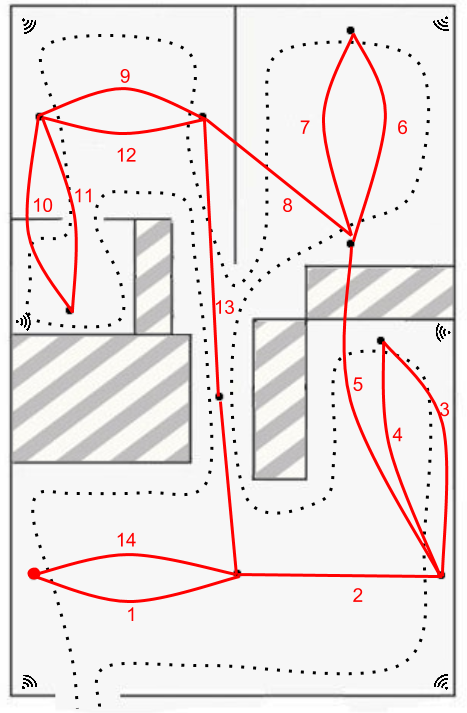
\includegraphics[width=2in,height=2.8in]{loc1_6ap_30s.png}
		\caption{Results with six access points and a thirty second polling time}
		\label{loc1_6ap_30s}
	\end{minipage}
\end{figure}


Figures \ref{loc1_4ap_10s} and \ref{loc1_6ap_10s} represent the two test variants with 10 second polling times. These variants are clearly quite susceptible to getting lost, particularly in the upper left quadrant of the map. Interestingly, both variants do seem to recover from their failure points, particularly in the upper right quadrant of the map. However, regardless of their recovery ability, both of these variants have significant issues with actual user locations and are not particularly useful as location estimators. 


Figures \ref{loc1_4ap_20s} and \ref{loc1_6ap_20s} represent the 20 second polling time variants. These are quite clearly far more accurate than the 10 second polling time variants. In Figure \ref{loc1_4ap_20s}, Honeycomb had a bit of trouble toward the upper middle section of the map at lines 6 and 7, but quickly recovered for the duration. Similarly, Figure \ref{loc1_6ap_20s} has an extra stopover at a fingerprint, represented by line 9, but also quickly recovered. It also has an aberration in which in line 13 goes straight to the end point, skipping a fingerprint in the middle of the map.

Figure \ref{loc1_4ap_30s} and \ref{loc1_6ap_30s} represent the 30 second polling time variants. Like the 20 second variants, both of these maps skip fingerprints a couple of times, but quickly recover and generally follow the correct movement trend. 